\documentclass[float=false, crop=true]{standalone}
\usepackage{import}
\usepackage{tikz}
\usepackage{pgfplots}
\usetikzlibrary{calc}
\usetikzlibrary{patterns}
%\usetikzlibrary{xfrac}
\usetikzlibrary{arrows}
\usetikzlibrary{shapes.geometric}
\pgfkeys{/pgf/number format/.cd,1000 sep={\,}}
\pgfplotsset{every tick label/.append style={font=\tiny}}

\begin{document}
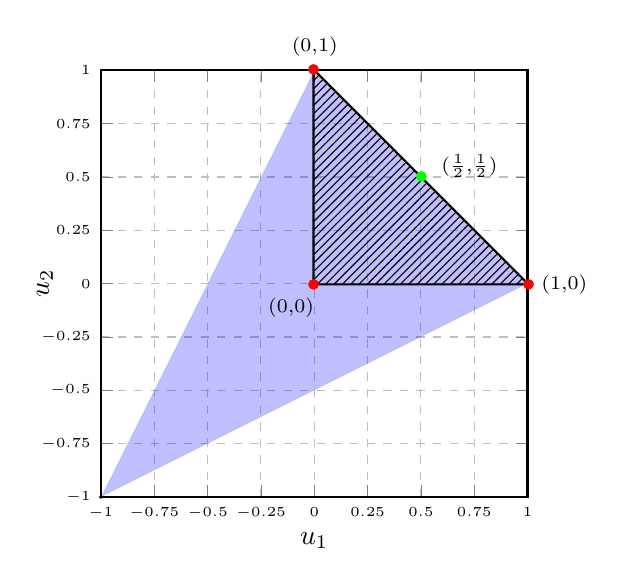
\begin{tikzpicture}
\begin{axis}[height=7cm,
    width=7cm,
    xlabel={$u_1$},
    ylabel={$u_2$},
    xmin=-1,
    xmax=1,
    ymin=-1,
    ymax=1,
    ylabel style={yshift=-0.40cm},
    xlabel style={yshift=0.08cm},
    scaled ticks=false, tick label style={/pgf/number format/fixed},
    xtick={-1, -0.75, -0.5, -0.25, 0, 0.25, 0.5, 0.75, 1},
    ytick={-1, -0.75, -0.5, -0.25, 0, 0.25, 0.5, 0.75, 1},
    no markers,
    line width=0.8pt,
    ymajorgrids=true,
    xmajorgrids=true,
    grid style=dashed,]
\end{axis}


% Correlated Strategies
\draw[black,fill=black] (0, 0) circle (.1ex) coordinate (1);
\draw[black,fill=black] (5.42, 2.71) circle (.1ex) coordinate (2);
\draw[black,fill=black] (2.71, 5.42) circle (.1ex) coordinate (3);
% Join them up
\fill [opacity=0.25,blue] (1) \foreach \i in {2,...,3}{ -- (\i) } -- cycle;


% Constrained Correlated Equilibrium Strategies
\draw[black,fill=black] (5.43, 2.7) circle (.0001ex) coordinate (1);
\draw[black,fill=black] (2.7, 2.7) circle (.0001ex) coordinate (2);
\draw[black,fill=black] (2.7, 5.43) circle (.0001ex) coordinate (8);
% Join them up
%\fill [opacity=0.25,red] (1) \foreach \i in {2,...,8}{ -- (\i) } -- cycle;
\draw[thick,black,pattern=north east lines,pattern color=black] (5.43, 2.7) -- (2.7, 2.7) -- (2.7, 5.43) -- (5.43, 2.7);

% Red Circles for Nash Equilibria
\draw[red,fill=red] (5.43, 2.7) circle (.4ex); % (1, 0)
\draw[red,fill=red] (2.7, 5.43) circle (.4ex); % (0, 1)
\draw[red,fill=red] (2.7, 2.7) circle (.4ex); % (0, 0)

% Correlated Equilibrium Circle
\draw[green,fill=green] (4.07, 4.07) circle (.4ex); % (1/2, 1/2)

% Text for Nash Equilibria
\node[anchor=west, right] at (5.47,2.7){$\scriptstyle (1,0)$};
\node[anchor=west, right] at (2.3,5.72){$\scriptstyle (0,1)$};
\node[anchor=west, right] at (4.2,4.2){$ \scriptstyle (\frac{1}{2}, \frac{1}{2})$};
\node[anchor=west, right] at (2,2.4){$ \scriptstyle (0,0)$};

\end{tikzpicture}


\end{document}
